\subsection{Data Understanding}

\subsubsection{Spotify}
Spotify is a music streaming service and has established itself as the Number one in this market. 
Since their launch in 2006, the company has gained over 365 million users, of which nearly 45 percent
are subscribed to the chargeable premium service. 
This Premium service comes at a subscription cost of nowadays 12,99€ per month,
giving the opportunity to listen to every song that is available at Spotify - this being
ca. 70 million tracks from over 1,2 million Artists.

Similar to other streaming services, Spotify also generates a lot of data.
The question here is how to filter out data from music in order to personalize user accounts. 
The founders evaluated millions of songs and taught an AI to independently recognize
patterns and certain structures within different genres. 
The results of the algorithm can be seen above all in the "Discovery Weekly Playlist". 
Users are presented with 30 songs that match their tastes here every Monday.
At the moment, the Spotify algorithm, which to this day goes by the name Echo Nest,
works because of three main components. 

First of all, it creates an individual Taste Profile for each Spotify user. 
There, it is recorded which artists, songs, albums, playlists and also podcast and audio books the
respective user listens to. 
And also how long he listens to the music tracks, where he does it and how often.
This data is then compared with the Taste Profiles of other users. 
For example, if another user has a large overlap in musical taste with your own playlists,
you will be shown songs in the Discovery Weekly playlist that the other user already listens to regularly.
Playlists with more followers end up in the Discovery Weekly folders more often than those with
fewer followers. 

In addition, the algorithm analyzes the individual components of the music tracks. 
It breaks down each song available on Spotify by tempo, instruments, duration, highs and lows,
timbre, and so on. 
Based on the large amount of data, the Spotify algorithm divides the songs into more than 1500
different genres so far. 
However, in addition to many regional differences in music genres, "nonsensical" genres keep
coming out in the AI's analysis. While it might be able to imagine something under deep power pop punk,
genres like djent are not really close to reality. 

This analysis step also includes the classification of songs into happy, sad,
melancholic or other types of music, so the classification according to feelings.
However, this feature is also controversial among experts, because there is no actual definition of sad or happy music. 
That always depends on the individual listener and his mood. To support the AI at this point,
it reads the titles of the playlists of the users. 
If a song often lands in playlists with titles like love songs or romantic music,
the AI assumes that the song is to be rated as a love song. 

At last, the Echo Nest algorithm searches the entire web daily for blog posts, comments on websites,
articles, YouTube videos, Facebook postings and comments and tweets, 
evaluates them, and uses them to create an opinion about a particular song.
Thus, within a few days, the algorithm notices how a song is received overall.  
This quickly creates a specific rating for each track, which in turn influences the
Discover function and other recommendation formats within the platform. 

\subsubsection{Feature analysis}
In the course of the analysis carried out here, three different genres were selected in order
to subsequently assign songs to the correct genre on the basis of the underlying data. 
The genres selected here are "Rock", "HipHop" and "Jazz". The selection was made under the original, 
subjective assumption that these genres differ particularly strongly in their characteristics and style. 
The assumption focused primarily on characteristics such as vocals, the general use of instruments,
the instruments used, or the energy of the songs of the respective genre.

The important insight for further consideration of the analysis is here:
Each genre that is considered, each song feature that is evaluated does not reflect reality, 
but only reflects the results of the Spotify algorithm. The analysis can,
according to subjective opinion, assign a Hip-Hop song to the category, 
or the genre Rock without being wrong - since the assignment makes sense based on the Spotify evaluations. 
Since the categories in the selected genres are very accurate due to their popularity,
the analysis is performed under the assumption that the two are congruent. 

As already mentioned, every song has given thirteen Features, which break down his main attributes into numbers.
To understand the data, it is crucial to get to know these features.
For a better presentation, they are divided into four clusters below, 
Musical Standards, Mood, Properties and Context.

\textbf{Musical Standards}

This Cluster includes the features, that capture and reflect the standard properties of music. 
These features are "Duration", "Key", "Mode" and "Time Signature". 
The feature “Duration”, as the name suggests, holds the information of how long the Track is.
This is measured in seconds. The feature “Key” is measured with an Integer between -1 and 11 and 
holds information about the key the track is in. Integers map to pitches using standard Pitch Class notation, E.g., 0 = C, 1 = C\(\sharp\) /D\(\flat\), 2 = D, and so on. 
If no key was detected, the value is -1.
“Mode” is an integer (either 0 or 1) and indicates the modality (major or minor) of a track. Major is represented by 1 and minor is 0. 
At last, the feature “Time Signature” is measured in an integer between 3 and 7.
It is a notational convention to specify how many beats are in each bar (or measure). 
The time signature ranges from 3 to 7 indicating time signatures of "3/4", to "7/4".

\textbf{Mood}

Following these features comes the cluster "Mood".
This cluster lists those features that measure the emotive values in songs, 
i.e. whether the song encourages dancing, spreads a positive or rather negative mood,
etc. This is captured with the features: "Danceability", "Valence", "Energy" and "Tempo".

All of these features except "Tempo" are measured in a float between 0 and 1. 
"Danceability" describes how suitable a track is for dancing based on a combination of musical elements
including tempo, rhythm stability, beat strength, and overall regularity. A value of 0.0 is least danceable and 1.0 is most danceable.
"Valence" describes the musical positiveness conveyed by a track. 
Tracks with high valence sound more positive (e.g. happy, cheerful, euphoric),
while tracks with low valence sound more negative (e.g. sad, depressed, angry).  
"Energy" represents a perceptual measure of intensity and activity. Typically, energetic tracks feel fast, loud, and noisy. 
A value near 1.0 indicates high energy, while tracks near 0.0 indicates low Values in this Feature. 
At last, "Tempo" holds the information about the overall estimated tempo of a track in beats per
minute (BPM). In musical terminology, tempo is the speed or pace of a given piece and derives directly from the
average beat duration.

\textbf{Properties}

This next cluster includes all features that capture the audio characteristics of the tracks,
such as "Loudness", "Speechiness" and "Instrumentalness".

"Loudness" is measured in a float number between -60 and 0 and measures the overall loudness
of a track in decibels (dB). 
The values are averaged across the entire track and are useful for comparing relative
loudness of tracks. 
"Speechiness", measured in a float number between 0 and 1, detects the presence of spoken words in a track. 
The more exclusively speech-like the recording (e.g. talk show, audio book, poetry),
the closer to 1.0 the attribute value. 
Values above 0.66 describe tracks that are probably made entirely of spoken words. Values below 0.33 most likely represent music and other non-speech-like tracks. 
"Instrumentalness", measured in a float between 0 and 1 as well, plays the counterpart to Speechiness.
It predicts whether a track contains no vocals at all. "Ooh" and "aah" sounds are treated as instrumental in this context.
The closer the Instrumentalness value is to 1.0, the more likely the track contains no vocal content. 
Values above 0.5 are intended to represent instrumental tracks, but confidence is higher as the value approaches 1.0.

\textbf{Context}

At last, this Cluster unions the Features “Liveness” and “Acousticness”.
These capture everything around the Songs, for example if it is played in front of a live audience.

Both Features are measured in a float number between 0 and 1.
Acousticness is a confidence measure from 0.0 to 1.0 of whether the track is acoustic. 1.0 represents high confidence the track is acoustic. 
Liveness detects the presence of an audience in the recording. 
Higher liveness values represent an increased probability that the track was performed live.
A value above 0.8 provides strong likelihood that the track is live. 

\subsubsection{Overall correlation}
After these explanations, the characteristics of the features in the individual categories are evaluated.
A correlation matrix is used for this purpose. This shows on a scale between 1 and -1 how
features correlate with each other. Since every song uses every feature,
a high correlation here does not mean that the features often appear together,
but how similar the values per song are. To start with an overall look over the data,
fig. 1  shows a genre independent matrix.
This means that the features of all songs that could be gathered in the step of data
collection were analyzed to create this figure. 

\begin{figure}[H]
    \centering
    \caption[]{Correlation matrix: categorie-independent correlation of features}
	\label{fig:du_cm_overall}
    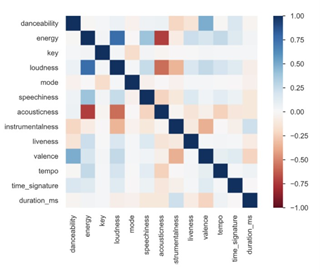
\includegraphics[width=0.4\textwidth]{output_overall.png}
\end{figure}

Generally, the features of the "Musical Standards" cluster can be ignored in this representation,
as they do not measure but only reflect characteristics (e.g., time signature or key).
It can be seen that "Energy" and "Loudness" have the highest correlation of the features,
with a value of approx. 0.65.  
%So, energetic songs often seem to be loud as well.
%This can be easily explained, since, as explained in the definition of the features:
%"Typically, energetic tracks feel fast, loud, and noisy".
In addition, there is a comparatively high correlation between "Valence" and "Dancebility" of
about 0.5. 
%which means that positive songs, i.e., songs with a high value for Valence,
%encourage more dancing than rather negative ones. 
The correlation between "Energy" and "Acousticness" is particularly negative, with a value of approx. -0.7.
%Acoustic tracks therefore often do not seem to be very energetic and vice versa.
The same can be said for "Accousticness" and "Loudness", with a correlation value of about -0.5.
Outside of these extreme values, the remaining correlation values settle between -0.2 and 0.2.
\textcolor{red}{Worth mentioning here are the correlations between "Instrumentalness" and "loudness" at
approx. -0.3 as well as "Instrumentalness" and Valence also at approx. -0.3. Furthermore,
in the positive "Speechiness" and "Energy" at a value of approx. 0.3.}

\begin{figure}[H]
    \centering
    \subfloat[\centering Correlation matrix: categorie Rock]{{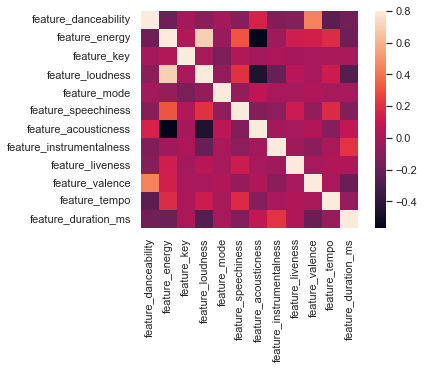
\includegraphics[width=4cm]{output_Rock.png} }}%
    \qquad
    \subfloat[\centering Correlation matrix: categorie HipHop]{{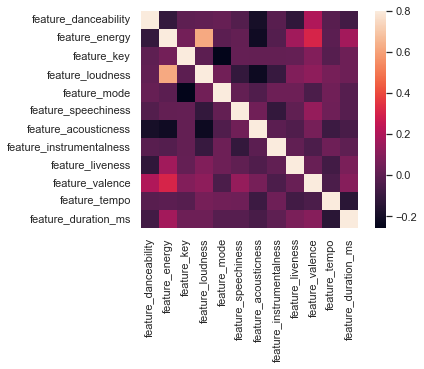
\includegraphics[width=4cm]{output_Hip_Hop.png} }}%
    \qquad
    \subfloat[\centering Correlation matrix: categorie Jazz]{{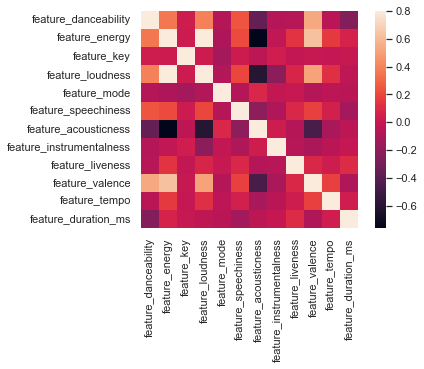
\includegraphics[width=4cm]{output_Jazz.png} }}%
    \caption{Correlations inside categories}%
    \label{fig:du_cm_categorie_dependent}%
\end{figure}

These correlations above now show the matrix on a category-specific basis.
It can be seen that the patterns described above also appear there.
However, the average correlation changes depending on the category.
For example, hip-hop has the same characteristics as the independent matrix category but shows
fundamentally more negative correlations (cf. Fig. 1 with Fig. 2 ).

\subsubsection{Correlation Music theorie - Data}
In the final step of Data Understanding,
the music theory described in the basic section is compared to the data used in the analysis.
This is necessary to develop a deeper understanding of the data.
As mentioned at the beginning of this chapter, theory and Spotify are not always necessarily congruent,
which is why a clear delineation is important here.
For this purpose, the properties of the genres in the music theory are tried to be compared
with the help of the features (e.g., "You can't dance well to rock" - What is the overall value for Danceability?).
To do this comparison, three features are chosen and discussed more deeply.
Subsequently, a better picture can be obtained with the help of further representations.

Starting with rock, one feature can be extracted here: The songs are mostly loud.
"Loudness" captures this property very well.
\textcolor{red}{It measures the actual, average loudness of a song in decibels, with most tracks falling
in the -60 to 0 range, where -60 is very quiet and 0 is very high.}
Overall, across all three categories, this feature has an average of -8.2544,
with a minimum value of -32.06 and a maximum value of 2.044.

\begin{figure}[H]
    \centering
    \subfloat[\centering Distribution plot: "Loudness"]{{\includegraphics[width=4cm]{output_loudness.png} }}%
    \qquad
    \subfloat[\centering Boxplot: "Loudness"]{{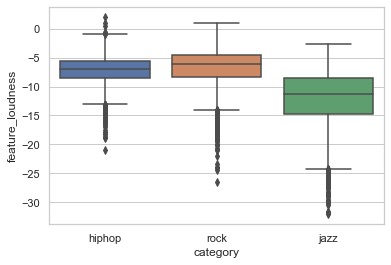
\includegraphics[width=4cm]{output_Loudness_boxplot.png} }}%
    \caption{"Loudness" compared in the different categories}%
    \label{fig:du_dp_bp_ln_categorie_dependent}%
\end{figure}

Figure 1  shows a so-called distribution plot.
The X-axis contains the scale of the feature used (in this case "loudness").
The Y-axis reflects the density of the respective category, meaning the more songs are found in the respective value, the higher the density.
As can be seen in the figure, all categories offer a very wide range of volume levels.
Jazz spreads its songs over an area from -32.06 (smallest value overall) to -2.695 but locates
most songs at about -10. Hip hop and rock go less wide but can accommodate more songs in the upper
quarter of the scale. Rock places its point furthest to the right of the scale.
Thus, it can be confirmed that rock can generally be classified as loud,
but also shows as the loudest of the three categories.
However, it must also be emphasized here that hip-hop comes shortly after.
In addition, jazz is not as loud as the other two categories, but it serves a much wider range. 

The next feature that can be scrutinized here is the large occurrence of instruments in jazz.
This can be checked in the Spotify data via the "Instrumentalness" feature.
\textcolor{red}{It measures the sole presence of instruments in songs with values between 0 and 1.
The closer the value approaches 1, the higher the probability that there are no vocals or other
elements in the song.} The overall average for this feature is 0.174.
The lowest value overall is 0.0 while the highest goes up to 0.989.

\begin{figure}[H]
    \centering
    \subfloat[\centering Distribution plot: "Instrumentalness"]{{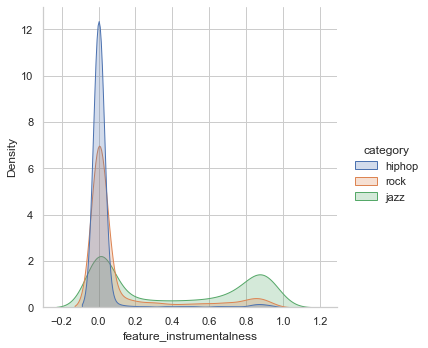
\includegraphics[width=4cm]{output_instumentelness.png} }}%
    \qquad
    \subfloat[\centering Boxplot: "Instrumentalness"]{{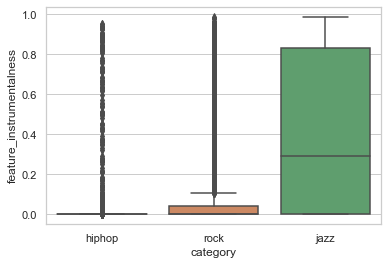
\includegraphics[width=4cm]{output_instumentelness_boxplot.png} }}%
    \caption{"Instrumentalness" compared in the different categories}%
    \label{du_dp_bp_instr_categorie_dependent}%
\end{figure}

For a better understanding, Figure x  also shows a distribution plot,
but adapted to the current feature.
It shows that both hip-hop and rock are almost exclusively found in the 0.0 - 0.1 range.
This means that songs in these categories almost only contain vocals.
However, slight increases in the range between 0.8 and 1.0 can also be seen. Jazz,
on the other hand, has two equally strong expressions. One in the range around 0.0,
the other between 0.8 and 1.0. Since jazz often contains only musical tracks without
any vocals, this reflects the reality quite well.
Here again, rock and hip-hop are similar in their high points.
In addition, jazz much differs from the two above. Again, it does not have such a high peak, 
but covers the scale much more broadly.

At last, a comparison of the categories in the "Energy" feature.
\textcolor{red}{Typically, energetic tracks feel fast, loud, and noisy.
The higher the value approaches 1, the more energetic it is.}
Basically, it is to be noted that there is a high average value of 0.65 overall.
This is clearer for rock with an average value of 0.7531.

\begin{figure}[H]
    \centering
    \subfloat[\centering Distribution plot: "Energy"]{{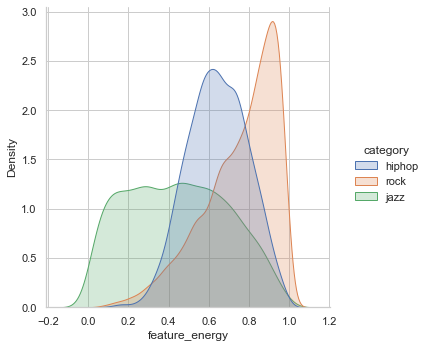
\includegraphics[width=4cm]{output_energy.png} }}%
    \qquad
    \subfloat[\centering Boxplot: "Energy"]{{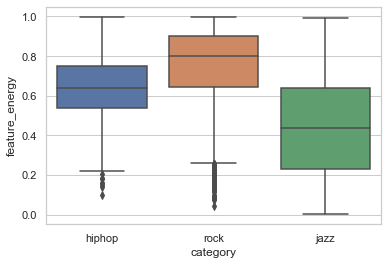
\includegraphics[width=4cm]{output_energy_boxplot.png} }}%
    \caption{"Energy" compared in the different categories}%
    \label{du_dp_bp_enrg_categorie_dependent}%
\end{figure}

If we now look at the data in a distribution plot (Figure x),
we see clear differences between the categories.
Jazz spreads over the whole graph but has no high point.
This can be attributed to the different types of jazz (slow jazz, free jazz),
which means that different subtypes have different levels of energy.
Surprisingly, HipHop is also broadly positioned and sets the high point at about 0.61.
HipHop also has many facets as a genre, which is why this expression also makes sense.
The curve of Rock builds up early but rises very steeply in the last third of the graph and marks
its high point at about 0.9. 

After these three sample features, some more distributions and boxplots are added to better
explain the characteristics of the individual genres.

\begin{figure}[H]
    \centering
    \subfloat[\centering Distribution plot: Speechiness]{{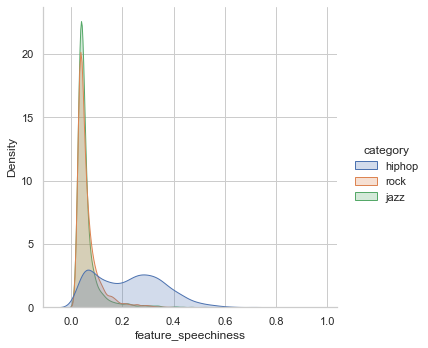
\includegraphics[width=4cm]{output_Speechiness.png} }}%
    \qquad
    \subfloat[\centering Boxplot: Speechiness]{{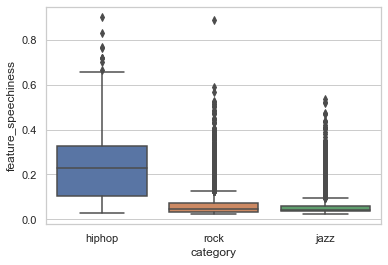
\includegraphics[width=4cm]{output_Speechiness_Boxplot.png} }}%
    \qquad
    \subfloat[\centering Distribution plot: Danceability]{{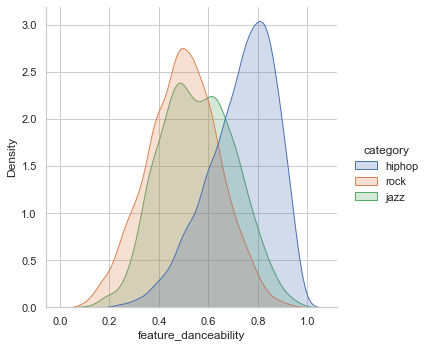
\includegraphics[width=4cm]{output_Danceability.png} }}%
    \qquad
    \subfloat[\centering Boxplot: Danceability]{{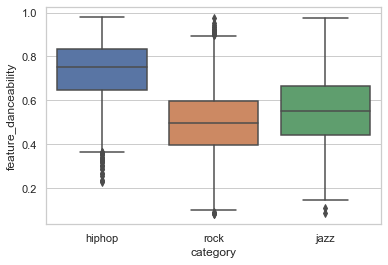
\includegraphics[width=4cm]{output_Danceability_Boxplot.png} }}%
    \qquad
    \subfloat[\centering Distribution plot: Accousticness]{{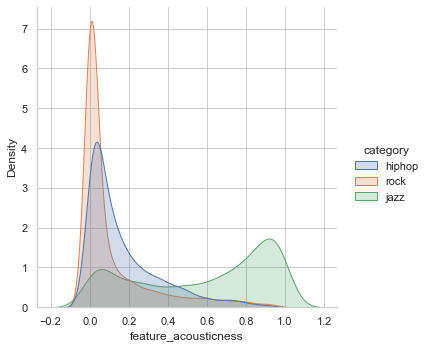
\includegraphics[width=4cm]{output_accousticness.png} }}%
    \qquad
    \subfloat[\centering Boxplot: Accousticness]{{\includegraphics[width=4cm]{output_accousticness_Boxplot.png} }}%
    \qquad
    \subfloat[\centering Distribution plot: Valence]{{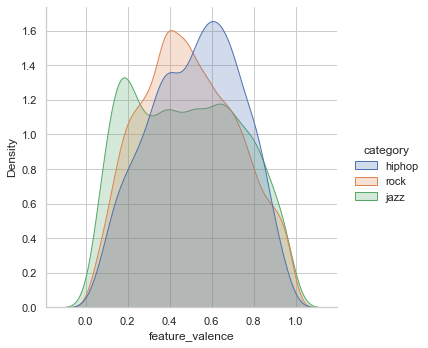
\includegraphics[width=4cm]{output_valence.png} }}%
    \qquad
    \subfloat[\centering Boxplot: Valence]{{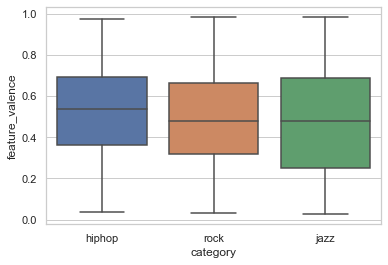
\includegraphics[width=4cm]{output_valence_Boxplot.png} }}%
    \qquad
    \caption{Different features visualized in distribution- and boxplots}%
    \label{fig:du_ds_bp_comparison}%
\end{figure}